\chapter{Página index.html}
La pagiona web que se utilizó para este ejercicio es un template que reutilicé de la asignatura pwm en angular, por lo que
no posee una estructura html tradicional, sino que se compone de un index.html y un main.js que se encarga de cargar el 
contenido dinámicamente. Para esta práctica, se ha modificado el index.html para incluir un mensaje de bienvenida y 
una breve descripción del servidor web seguro que se ha configurado. Además, se han ajustado los permisos del archivo para 
asegurar que el servidor Apache pueda acceder a él correctamente. No se han realizado otras modificaciones adicionales en la 
configuración del servidor para esta parte de la práctica. Sin embargo, hay una corrección ya que en el capitulo 2 debí
de haber configurado el a2enmod ssl para habilitar el módulo SSL en Apache pero debido a que trabajo en dos equipos diferentes,
en mi equipo portatil no lo tenía habilitado.
\section{Enunciado}
6. Creación y configuración del fichero \texttt{index.html}. Permisos y configuración adicional necesaria.
\section{Resolución}
Una vez el código angular estaba terminado:
\begin{lstlisting}[language=html, caption={Página index.html del servidor web}]
    <!-- ═══════════════════════════════════════════════════════════
     Seguridad de la Información & Criptografía
     ═══════════════════════════════════════════════════════════ -->

<!-- ── NAVIGATION ── -->
<nav class="navbar">
  <div class="nav-container">
    <a class="nav-brand" (click)="scrollTo('inicio')">
      <span class="brand-icon">🛡️</span>
      <span class="brand-text">CryptoSI</span>
    </a>
    <button class="nav-toggle" (click)="toggleMenu()" [attr.aria-expanded]="mobileMenuOpen()">
      <span class="hamburger" [class.active]="mobileMenuOpen()"></span>
    </button>
    <ul class="nav-links" [class.open]="mobileMenuOpen()">
      @for (section of sections; track section.id) {
        <li>
          <a (click)="scrollTo(section.id)">{{ section.label }}</a>
        </li>
      }
    </ul>
  </div>
</nav>

<!-- ── HERO ── -->
<section id="inicio" class="hero">
  <div class="hero-bg">
    <div class="grid-overlay"></div>
    <div class="glow glow-1"></div>
    <div class="glow glow-2"></div>
    <div class="floating-code">
      <span class="code-line"><span class="kw">const</span> key = <span class="fn">crypto</span>.<span class="fn">generateKey</span>(<span class="str">'AES-256'</span>);</span>
      <span class="code-line"><span class="kw">const</span> cipher = <span class="fn">encrypt</span>(plaintext, key);</span>
      <span class="code-line"><span class="cm">// 🔒 Datos protegidos</span></span>
    </div>
  </div>
  <div class="hero-content">
    <div class="hero-badge">
      <span class="badge-dot"></span>
      Seguridad de la Información
    </div>
    <h1 class="hero-title">
      Protege tus datos con
      <span class="gradient-text">Criptografía</span>
    </h1>
    <p class="hero-subtitle">
      Explora los fundamentos de la seguridad informática: cifrado simétrico, asimétrico,
      funciones hash, certificados digitales y más.
    </p>
    <div class="hero-actions">
      <button class="btn btn-primary" (click)="scrollTo('temas')">
        Explorar Temas
        <span class="btn-arrow">→</span>
      </button>
      <button class="btn btn-secondary" (click)="scrollTo('demo')">
        Demo Interactiva
      </button>
    </div>
    <div class="hero-stats">
      <div class="stat">
        <span class="stat-number">256</span>
        <span class="stat-label">bits AES</span>
      </div>
      <div class="stat-divider"></div>
      <div class="stat">
        <span class="stat-number">4096</span>
        <span class="stat-label">bits RSA</span>
      </div>
      <div class="stat-divider"></div>
      <div class="stat">
        <span class="stat-number">SHA</span>
        <span class="stat-label">-512 Hash</span>
      </div>
    </div>
  </div>
</section>

<!-- ── TOPICS GRID ── -->
<section id="temas" class="section">
  <div class="container">
    <div class="section-header">
      <span class="section-tag">Fundamentos</span>
      <h2 class="section-title">Pilares de la Seguridad</h2>
      <p class="section-subtitle">
        La criptografía es la base de la seguridad digital moderna. Conoce los conceptos clave.
      </p>
    </div>
    <div class="topics-grid">
      @for (topic of topics; track topic.title) {
        <div class="topic-card" [attr.data-color]="topic.color">
          <div class="topic-icon">{{ topic.icon }}</div>
          <h3>{{ topic.title }}</h3>
          <p>{{ topic.desc }}</p>
          <div class="topic-tags">
            @for (alg of topic.algorithms; track alg) {
              <span class="tag">{{ alg }}</span>
            }
          </div>
        </div>
      }
    </div>
  </div>
</section>

<!-- ── SYMMETRIC ENCRYPTION ── -->
<section id="cifrado-simetrico" class="section section-alt">
  <div class="container">
    <div class="section-header">
      <span class="section-tag">Cifrado Simétrico</span>
      <h2 class="section-title">Una clave, dos operaciones</h2>
      <p class="section-subtitle">
        El cifrado simétrico utiliza la misma clave secreta tanto para cifrar como para descifrar.
        Es rápido y eficiente para grandes volúmenes de datos.
      </p>
    </div>

    <div class="symmetric-flow">
      <div class="flow-step">
        <div class="flow-icon">📄</div>
        <span>Texto plano</span>
      </div>
      <div class="flow-arrow">+</div>
      <div class="flow-step highlight">
        <div class="flow-icon">🔑</div>
        <span>Clave secreta</span>
      </div>
      <div class="flow-arrow">→</div>
      <div class="flow-step">
        <div class="flow-icon">🔒</div>
        <span>Texto cifrado</span>
      </div>
      <div class="flow-arrow">+</div>
      <div class="flow-step highlight">
        <div class="flow-icon">🔑</div>
        <span>Misma clave</span>
      </div>
      <div class="flow-arrow">→</div>
      <div class="flow-step">
        <div class="flow-icon">📄</div>
        <span>Texto original</span>
      </div>
    </div>

    <div class="algorithms-grid">
      @for (alg of symmetricAlgorithms; track alg.name) {
        <div class="algorithm-card">
          <div class="alg-header">
            <span class="alg-name">{{ alg.name }}</span>
            <span class="alg-badge">{{ alg.security }}</span>
          </div>
          <p class="alg-fullname">{{ alg.fullName }}</p>
          <p class="alg-desc">{{ alg.desc }}</p>
          <div class="alg-specs">
            <div class="spec">
              <span class="spec-label">Clave</span>
              <span class="spec-value">{{ alg.keySize }}</span>
            </div>
            <div class="spec">
              <span class="spec-label">Bloque</span>
              <span class="spec-value">{{ alg.blockSize }}</span>
            </div>
          </div>
          <div class="alg-modes">
            @for (mode of alg.modes; track mode) {
              <span class="mode-tag">{{ mode }}</span>
            }
          </div>
        </div>
      }
    </div>
  </div>
</section>

<!-- ── ASYMMETRIC ENCRYPTION ── -->
<section id="cifrado-asimetrico" class="section">
  <div class="container">
    <div class="section-header">
      <span class="section-tag">Cifrado Asimétrico</span>
      <h2 class="section-title">El poder de dos claves</h2>
      <p class="section-subtitle">
        La criptografía de clave pública revolucionó la seguridad al eliminar la necesidad de
        compartir secretos previamente.
      </p>
    </div>

    <div class="asymmetric-grid">
      @for (concept of asymmetricConcepts; track concept.title) {
        <div class="asymmetric-card">
          <div class="asym-icon">{{ concept.icon }}</div>
          <h3>{{ concept.title }}</h3>
          <p>{{ concept.desc }}</p>
        </div>
      }
    </div>

    <div class="rsa-demo">
      <h3 class="rsa-title">Proceso RSA simplificado</h3>
      <div class="rsa-steps">
        <div class="rsa-step">
          <div class="step-number">1</div>
          <div class="step-content">
            <strong>Generación de claves</strong>
            <p>Se eligen dos primos grandes <em>p</em> y <em>q</em>, se calcula <em>n = p × q</em> y se obtiene el par de claves.</p>
          </div>
        </div>
        <div class="rsa-step">
          <div class="step-number">2</div>
          <div class="step-content">
            <strong>Cifrado</strong>
            <p>El emisor cifra con la clave pública del receptor: <code>C = M^e mod n</code></p>
          </div>
        </div>
        <div class="rsa-step">
          <div class="step-number">3</div>
          <div class="step-content">
            <strong>Descifrado</strong>
            <p>El receptor descifra con su clave privada: <code>M = C^d mod n</code></p>
          </div>
        </div>
      </div>
    </div>
  </div>
</section>

<!-- ── HASH FUNCTIONS ── -->
<section id="hash" class="section section-alt">
  <div class="container">
    <div class="section-header">
      <span class="section-tag">Funciones Hash</span>
      <h2 class="section-title">Huellas digitales únicas</h2>
      <p class="section-subtitle">
        Las funciones hash convierten datos de cualquier tamaño en una cadena de longitud fija,
        siendo prácticamente imposible revertir el proceso.
      </p>
    </div>

    <div class="hash-properties">
      <div class="hash-prop">
        <div class="prop-icon">🎯</div>
        <h4>Determinista</h4>
        <p>La misma entrada siempre produce la misma salida.</p>
      </div>
      <div class="hash-prop">
        <div class="prop-icon">⚡</div>
        <h4>Rápida</h4>
        <p>El cálculo del hash se realiza en tiempo eficiente.</p>
      </div>
      <div class="hash-prop">
        <div class="prop-icon">🚫</div>
        <h4>Irreversible</h4>
        <p>No se puede obtener la entrada a partir del hash.</p>
      </div>
      <div class="hash-prop">
        <div class="prop-icon">🔀</div>
        <h4>Efecto Avalancha</h4>
        <p>Un cambio mínimo en la entrada cambia drásticamente el hash.</p>
      </div>
    </div>

    <div class="hash-comparison">
      <h3>Comparativa de algoritmos</h3>
      <div class="hash-table-wrapper">
        <table class="hash-table">
          <thead>
            <tr>
              <th>Algoritmo</th>
              <th>Salida (bits)</th>
              <th>Estado</th>
              <th>Uso</th>
            </tr>
          </thead>
          <tbody>
            <tr>
              <td><span class="algo-name">MD5</span></td>
              <td>128</td>
              <td><span class="status-badge danger">Inseguro</span></td>
              <td>Checksums (legacy)</td>
            </tr>
            <tr>
              <td><span class="algo-name">SHA-1</span></td>
              <td>160</td>
              <td><span class="status-badge warning">Débil</span></td>
              <td>Git (legacy)</td>
            </tr>
            <tr>
              <td><span class="algo-name">SHA-256</span></td>
              <td>256</td>
              <td><span class="status-badge success">Seguro</span></td>
              <td>TLS, Bitcoin, certificados</td>
            </tr>
            <tr>
              <td><span class="algo-name">SHA-512</span></td>
              <td>512</td>
              <td><span class="status-badge success">Seguro</span></td>
              <td>Firmas digitales, contraseñas</td>
            </tr>
            <tr>
              <td><span class="algo-name">Whirlpool</span></td>
              <td>512</td>
              <td><span class="status-badge success">Seguro</span></td>
              <td>Integridad de datos</td>
            </tr>
          </tbody>
        </table>
      </div>
    </div>
  </div>
</section>

<!-- ── INTERACTIVE DEMO ── -->
<section id="demo" class="section">
  <div class="container">
    <div class="section-header">
      <span class="section-tag">Laboratorio</span>
      <h2 class="section-title">Demo Interactiva</h2>
      <p class="section-subtitle">Prueba los conceptos criptográficos en tiempo real.</p>
    </div>

    <div class="demos-grid">
      <!-- Caesar Cipher -->
      <div class="demo-card">
        <div class="demo-header">
          <span class="demo-icon">🔄</span>
          <h3>Cifrado César</h3>
        </div>
        <p class="demo-desc">
          Uno de los cifrados más antiguos. Desplaza cada letra del alfabeto un número fijo de posiciones.
        </p>
        <div class="demo-controls">
          <label>
            <span class="input-label">Texto original</span>
            <input
              type="text"
              [ngModel]="caesarInput()"
              (ngModelChange)="caesarInput.set($event)"
              placeholder="Escribe algo…"
              class="demo-input"
            />
          </label>
          <label>
            <span class="input-label">Desplazamiento: {{ caesarShift() }}</span>
            <input
              type="range"
              min="1"
              max="25"
              [ngModel]="caesarShift()"
              (ngModelChange)="caesarShift.set(+$event)"
              class="demo-range"
            />
          </label>
        </div>
        <div class="demo-result">
          <span class="result-label">Resultado cifrado</span>
          <div class="result-value mono">{{ caesarOutput() }}</div>
        </div>
      </div>

      <!-- SHA-256 Hash -->
      <div class="demo-card">
        <div class="demo-header">
          <span class="demo-icon">🧬</span>
          <h3>Hash SHA-256</h3>
        </div>
        <p class="demo-desc">
          Genera la huella digital SHA-256 de cualquier texto usando la Web Crypto API del navegador.
        </p>
        <div class="demo-controls">
          <label>
            <span class="input-label">Texto a hashear</span>
            <input
              type="text"
              [ngModel]="hashInput()"
              (ngModelChange)="hashInput.set($event)"
              placeholder="Escribe algo…"
              class="demo-input"
            />
          </label>
          <button class="btn btn-primary btn-sm" (click)="computeHash()">
            Calcular SHA-256
          </button>
        </div>
        @if (hashOutput()) {
          <div class="demo-result">
            <span class="result-label">Hash SHA-256</span>
            <div class="result-value mono hash-output">{{ hashOutput() }}</div>
          </div>
        }
      </div>
    </div>
  </div>
</section>

<!-- ── FOOTER ── -->
<footer class="footer">
  <div class="container">
    <div class="footer-content">
      <div class="footer-brand">
        <span class="brand-icon">🛡️</span>
        <span class="brand-text">CryptoSI</span>
      </div>
      <p class="footer-text">
        Práctica 6 — Seguridad de la Información · ULPGC 2025-26
      </p>
      <div class="footer-links">
        <span>Hecho con Angular &amp; ❤️</span>
      </div>
    </div>
  </div>
</footer>
\end{lstlisting}

Una vez creada la pagina, se compila utilizando:
\begin{lstlisting}[language=bash]
ng build --prod
\end{lstlisting}
Y se copia el contenido de la carpeta \texttt{dist} al directorio raíz del servidor web, asegurándose de que los permisos 
sean correctos para que Apache pueda servir los archivos sin problemas.

\begin{figure}
    \centering
    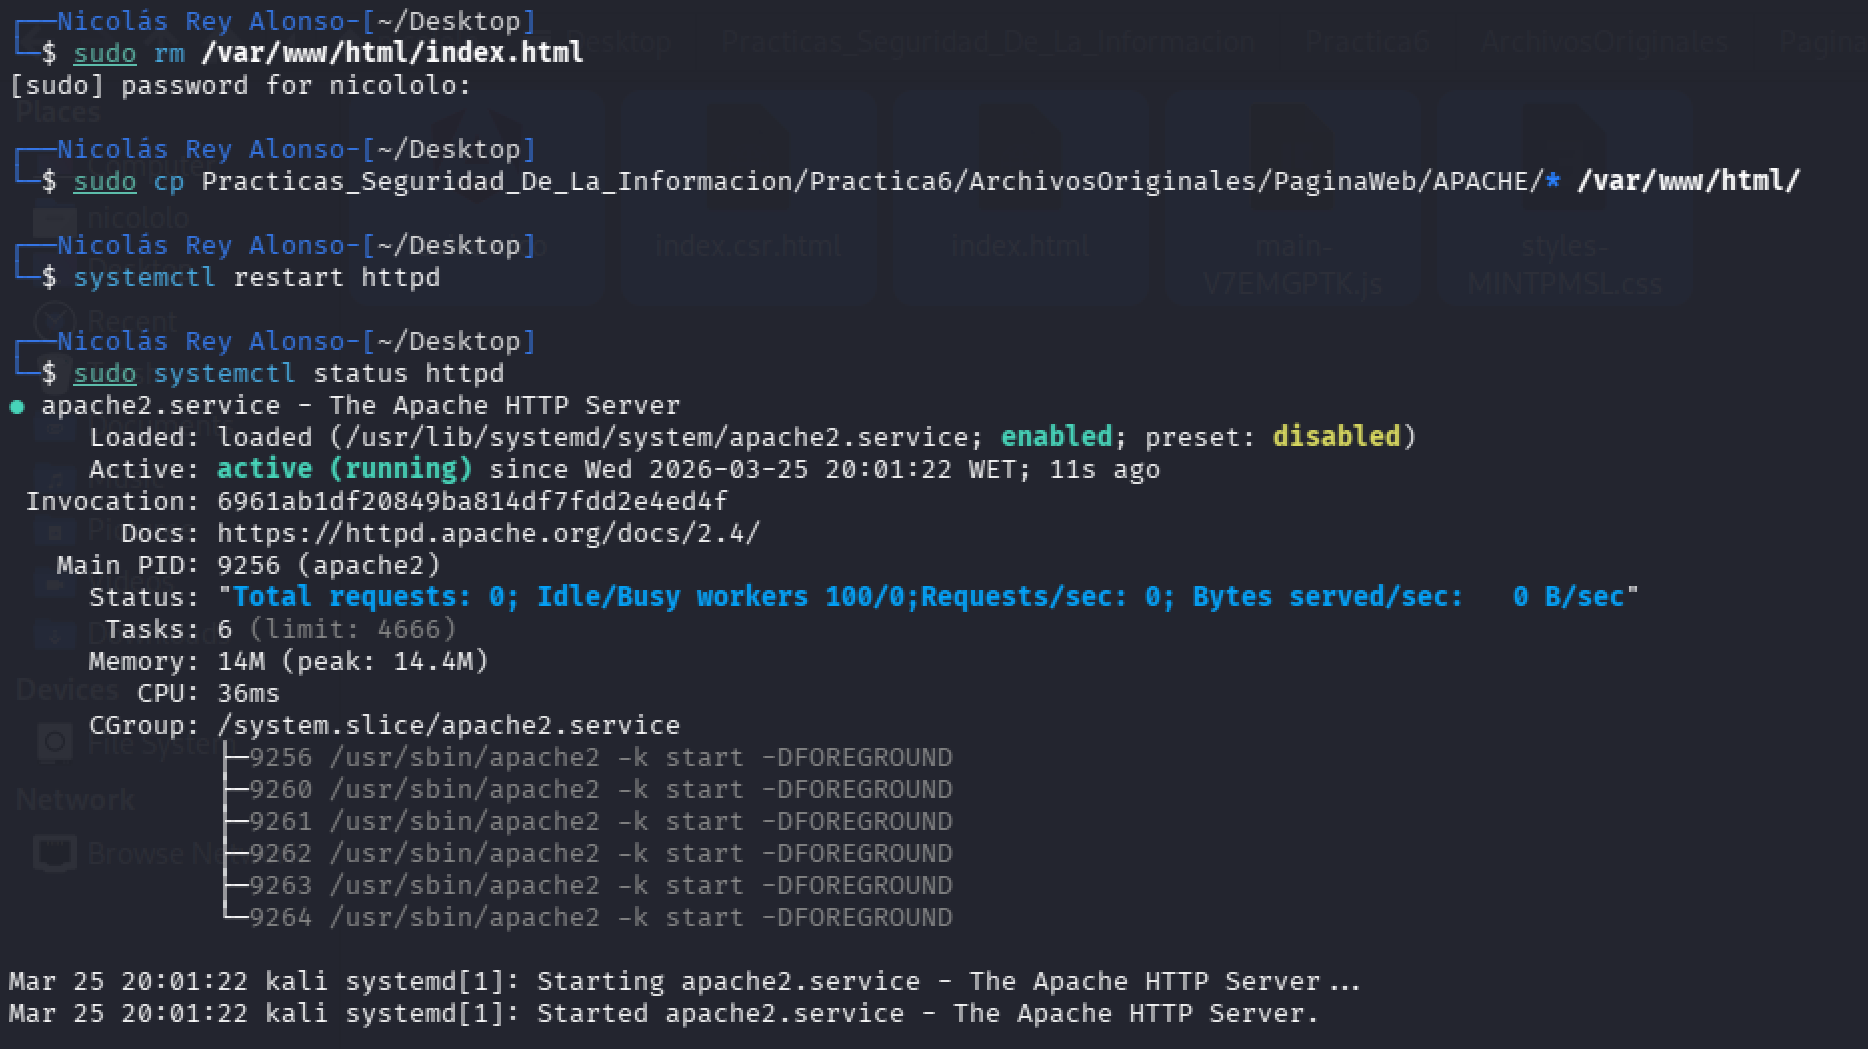
\includegraphics[width=0.8\textwidth]{Imagenes/14.png}
    \caption{Copiado del contenido de dist al directorio raíz del servidor web}
\end{figure}
